
\documentclass[t, 11pt]{beamer}
%\pdfmapfile{+sansmathaccent.map}
%%% Работа с русским языком
\usepackage{cmap}				
\usepackage{mathtext} 				
\usepackage[T2A]{fontenc}		
\usepackage[utf8]{inputenc}			
\usepackage[russian, english]{babel}	

\usetheme{Montpellier}
\usecolortheme{beaver} % Цветовая схема

\usepackage{advdate}



%%% Работа с картинками
\usepackage{graphicx}

\usepackage{csquotes}

\hypersetup{				
	colorlinks=true,       	
	linkcolor=blue,          
	citecolor=black,       
	filecolor=magenta,      
	urlcolor=red           
}
%% табличка
\usepackage{booktabs, caption, makecell}
\usepackage{threeparttable}

%% график нормального распределения 
\usepackage{tikz}
\usepackage{xcolor}
\usepackage{pgfplots}
\pgfplotsset{compat=1.7}

%% доп символы
\usepackage{newunicodechar}

\newcommand\Warning{%
	\makebox[1.4em][c]{%
		\makebox[0pt][c]{\raisebox{.1em}{\small!}}%
		\makebox[0pt][c]{\color{red}\Large$\bigtriangleup$}}}%

%\newunicodechar{⚠}{\Warning}

\title {GLM}
\subtitle{Advanced regression}
\author{Chuvakin Sergey}
\date{\today}
\institute[<<Anthropology and Sociology major>>]{<<School of Advanced Studies>>}

\begin{document}
	
	
	\frame[plain]{\titlepage}		
	
	\section{Outline}
	
	\begin{frame} 
		\frametitle{\insertsection} 
		\begin{itemize}
			\item Assumptions
			\item Normal distribution
			\item types 
			\item link function
			\item logit
			\item estimators
			\item probit (normal distribution)
			\item interpretation
		\end{itemize}
		
	\end{frame}
	
	\section{Assumptions}
		\begin{frame} 
		\frametitle{\insertsection} 
	\begin{itemize}
			\item Linearity of data
			\item Sample should be \emph{randomly} selected for population
			\item X matrix should not be correlated within
			\item X marrix should not be correlated with error
			\item Variance of error should be constant
			\item \emph{Normality of Y}
\end{itemize}

	\end{frame}
\section{Normall Distribution}
	
			\begin{frame} 
		\frametitle{\insertsection} 
		\begin{center}
			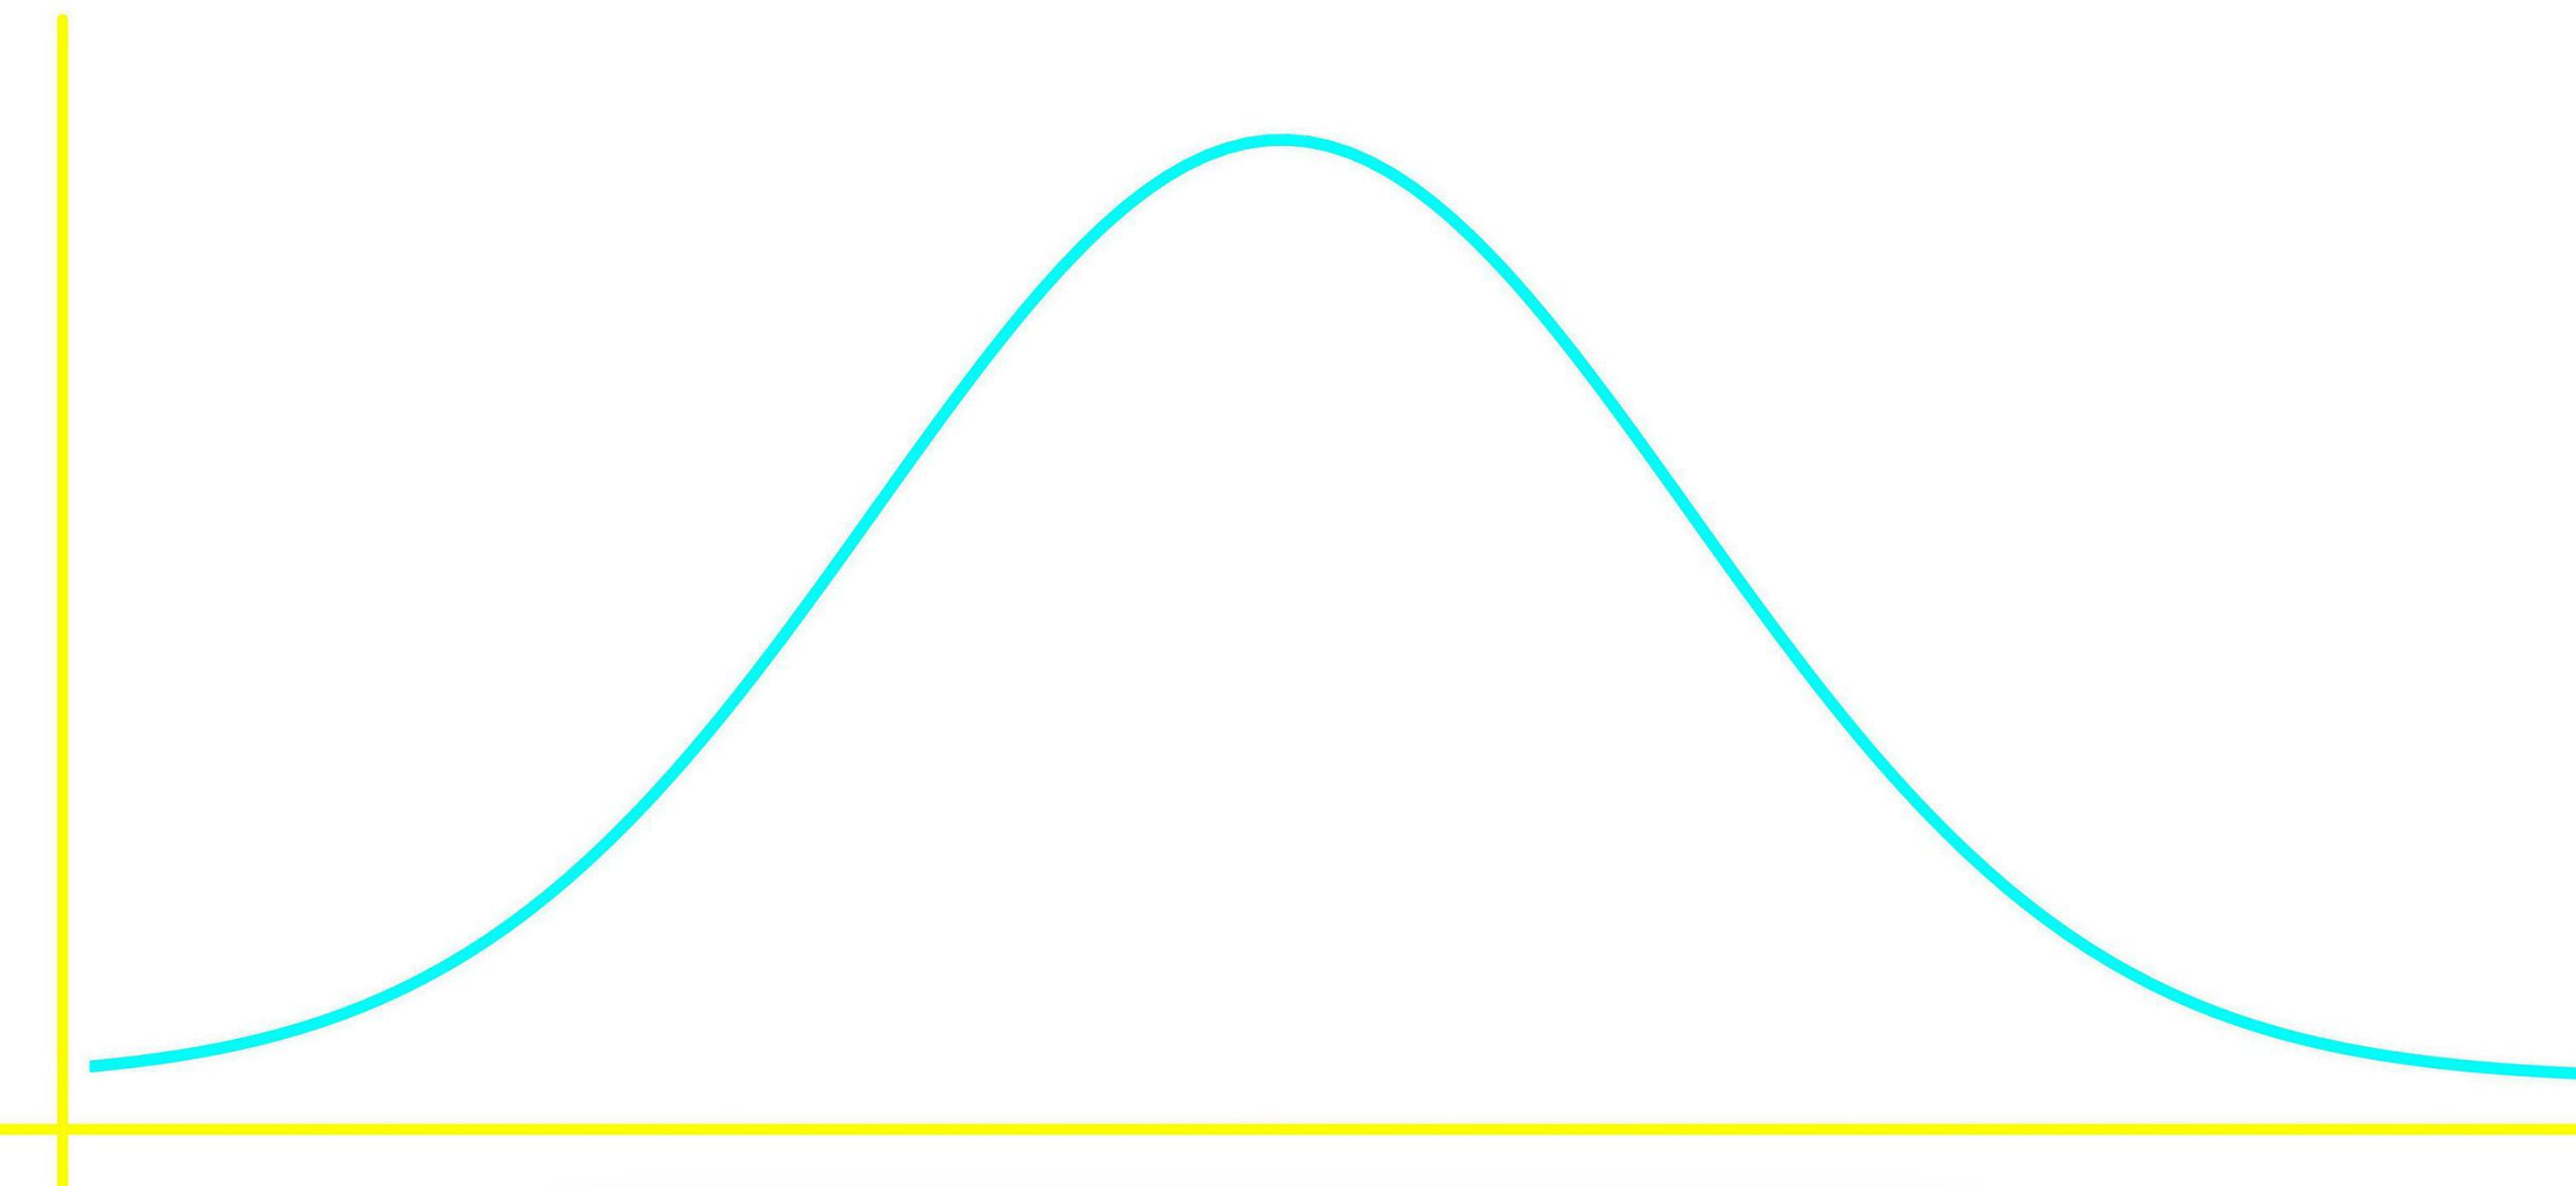
\includegraphics[scale=0.2]{bellshape}
		\end{center}
	\end{frame}
\section{Types}

\begin{frame} 
	\frametitle{\insertsection} 
	\begin{center}
		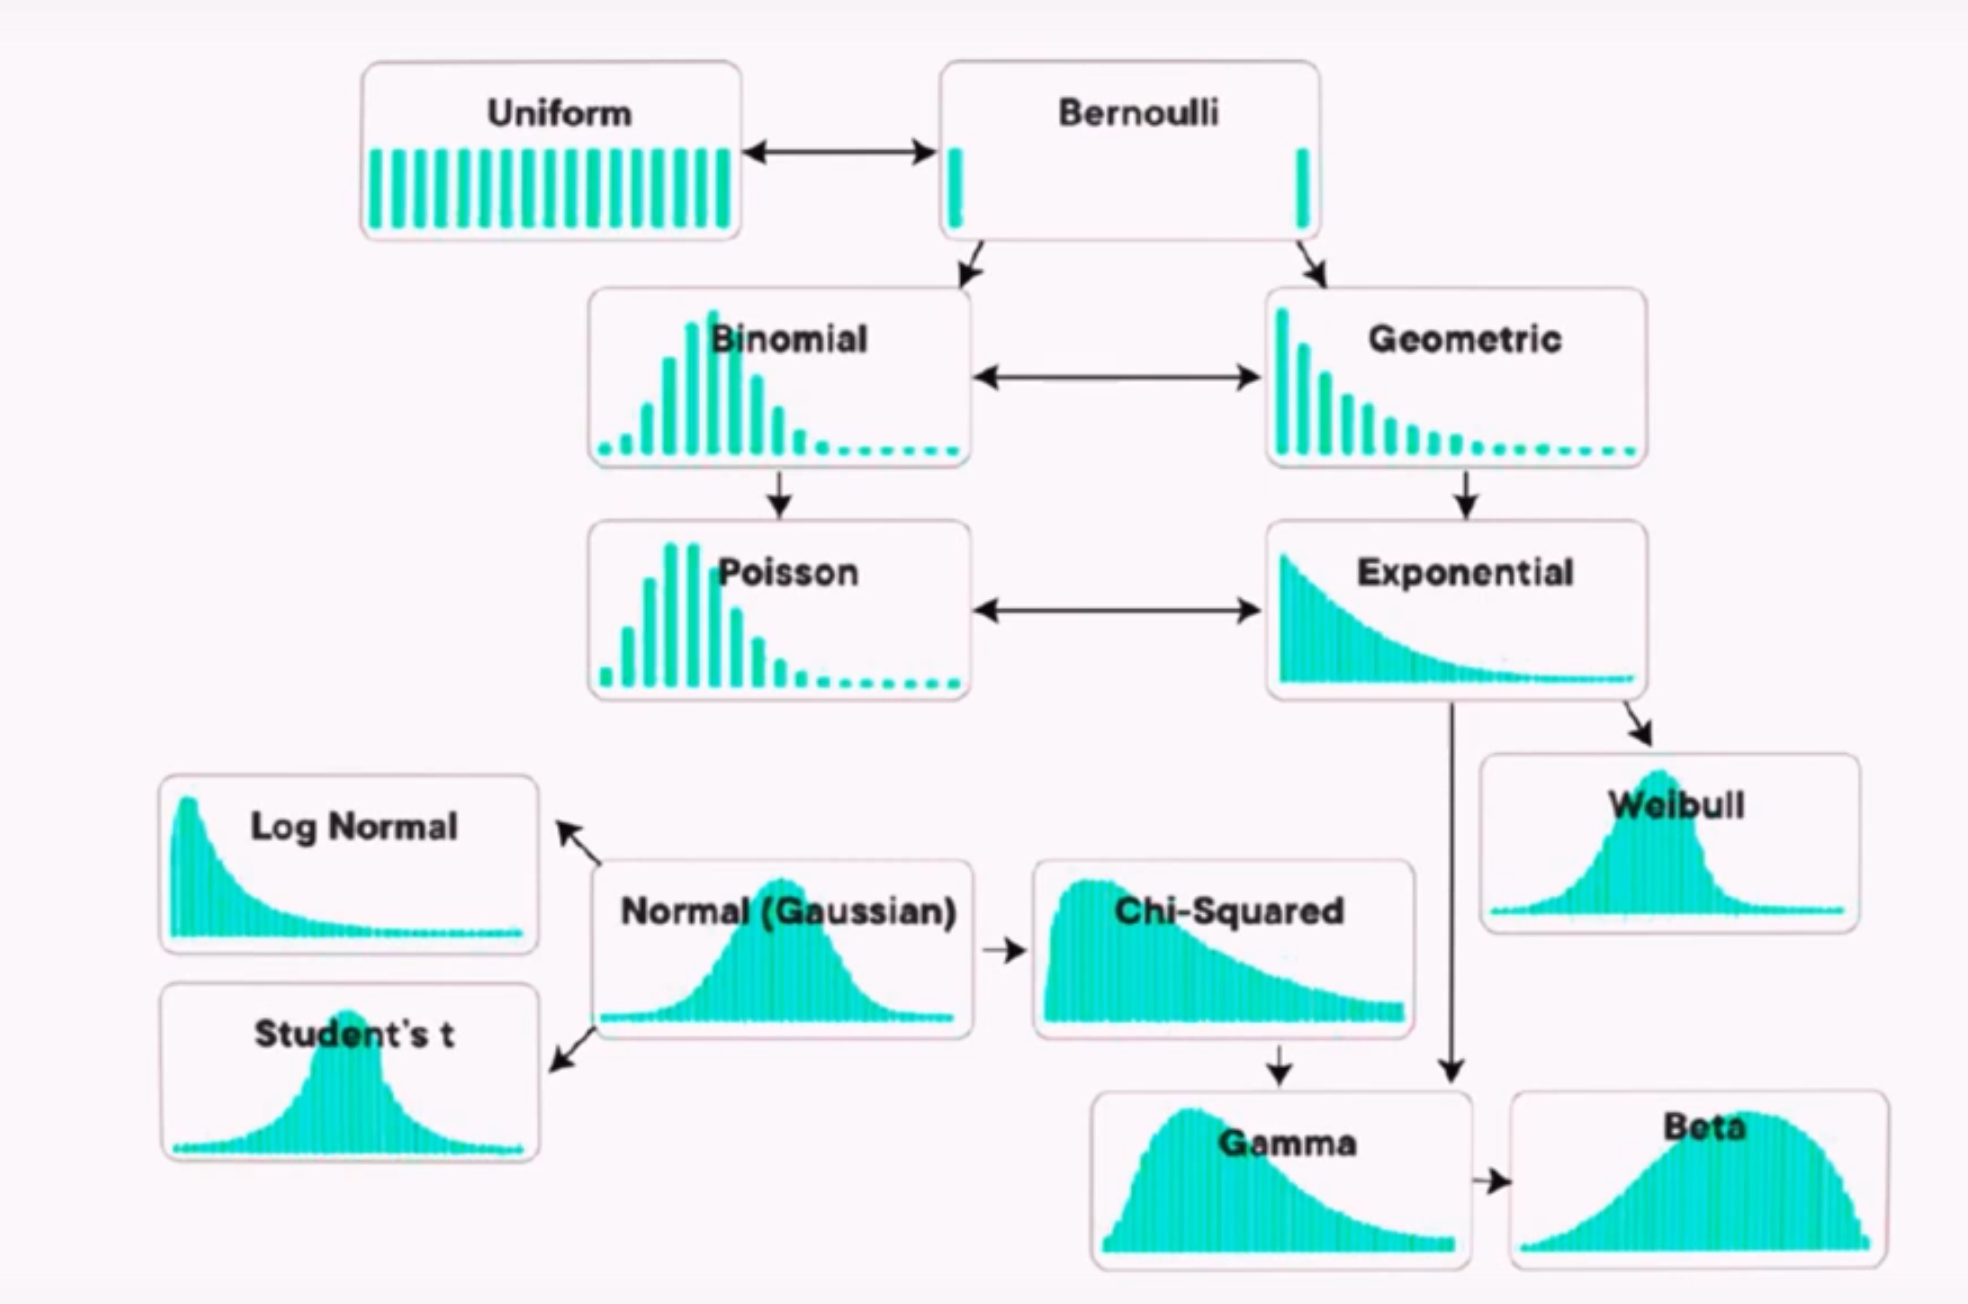
\includegraphics[scale=0.3]{varaity}
	\end{center}
\end{frame}	

\section{Idea}

\begin{frame} 
	\frametitle{\insertsection} 
	\begin{center}
		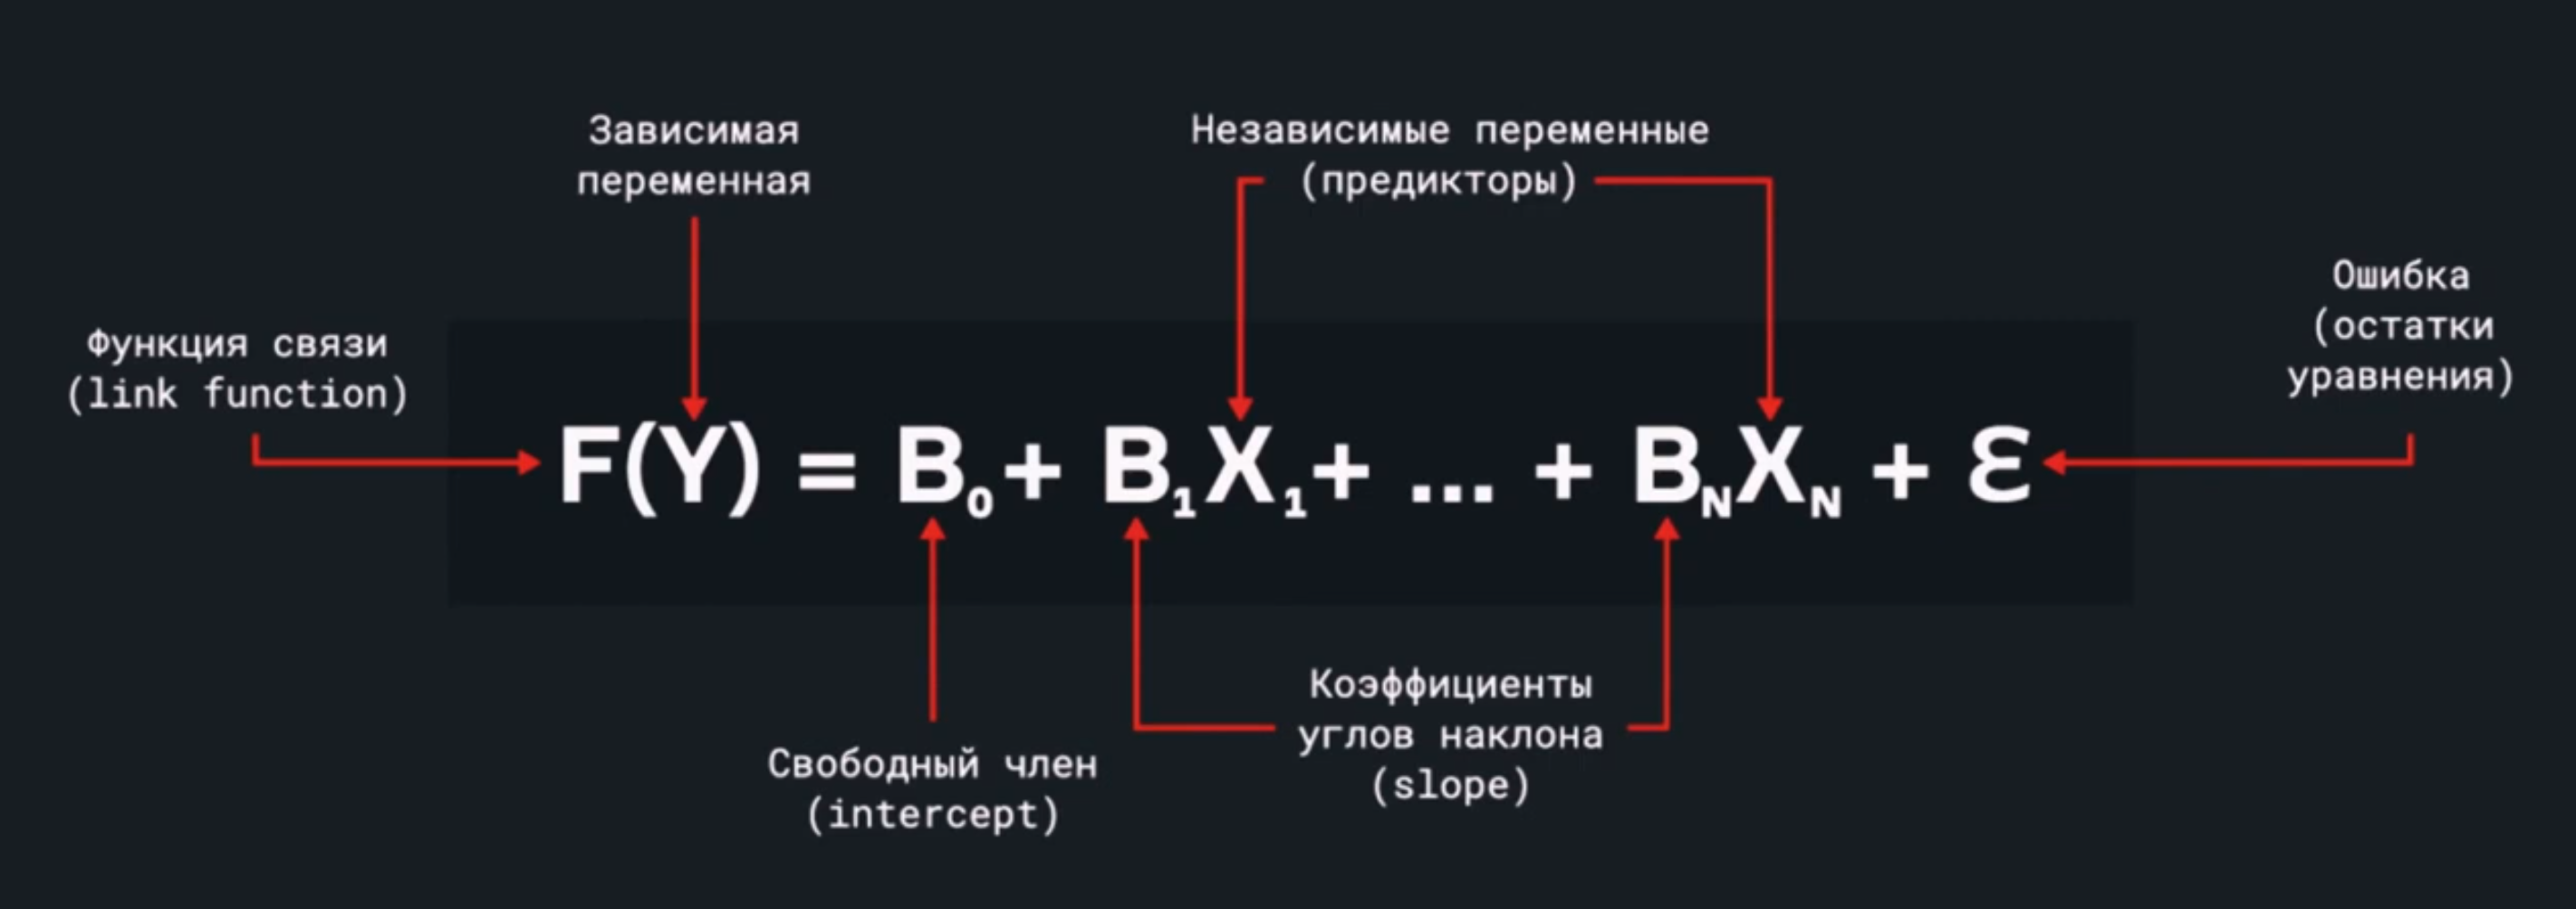
\includegraphics[scale=0.23]{formula}
	\end{center}
\end{frame}	
	
\section{Link functons}
	
	\begin{frame} 
		\frametitle{\insertsection} 
		\begin{itemize}
			\item Identity
			\item log (logit)
			\item probit
			\item poisson
			\item negative binomial
			\item etc
		\end{itemize}
	\end{frame}	

\section{Logit}
	
	\begin{frame} 
		\frametitle{\insertsection} 
	This type of regression suits for binary varaible.  
	\begin{center}
		\begin{equation}
			Y = log(\frac{p}{1 -p})
		\end{equation}
	\end{center}
	Coef output not an absolute straightforward number to interpret - it's a chance. 
	
	Chance is a probability relation. 1 means that there is equal probability for success and for fail.  
	\end{frame}	

\begin{frame}
	\frametitle{\insertsection} 
\begin{center}
	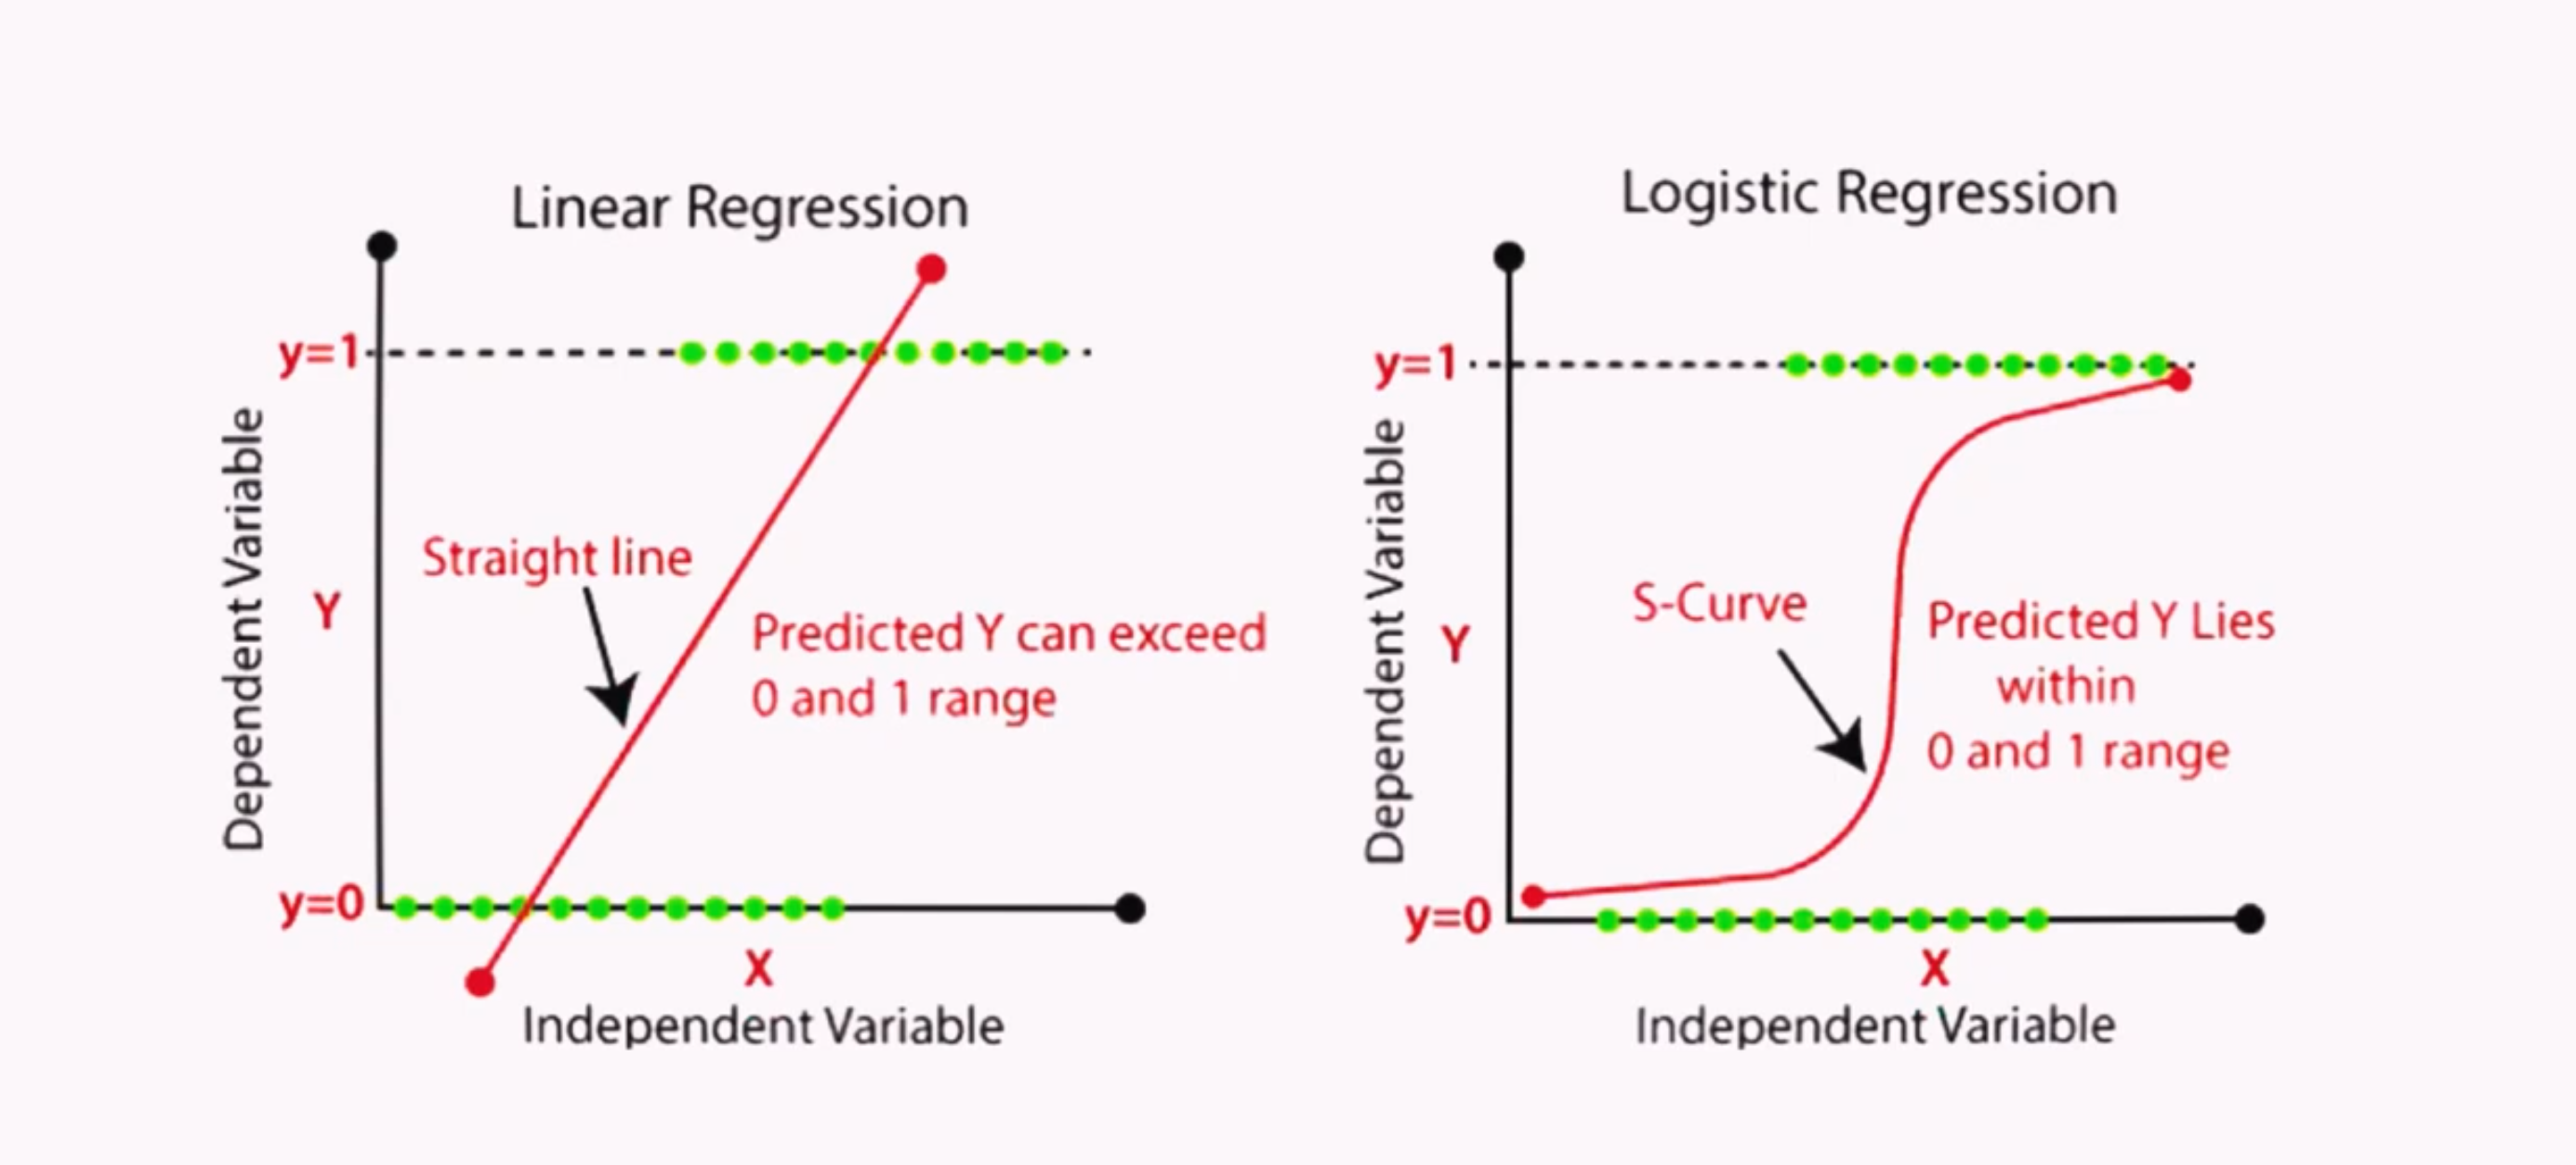
\includegraphics[scale=0.23]{logit}
\end{center}
\end{frame}	



	\section{Estimator}
\begin{frame} 
	\frametitle{\insertsection} 
	MLE  - Maximul likelihood Estimator more suits to logit and other GLM
	\begin{center}
		\begin{equation}
			\text{likelihood} = \hat{y} * y + (1 – \hat{y}) * (1 – y)
		\end{equation}
		\begin{equation}
		\text{log-likelihood} = log(\hat{y}) * y + log(1 – \hat{y}) * (1 – y)
	\end{equation}
		\begin{equation}
	\text{maximize: } \Sigma^n_i  log(\hat{y_i}) * y_i + log(1 – \hat{y_i}) * (1 – y_i)
\end{equation}
		\begin{equation}
	\text{minimize: } \Sigma^n_i  -(log(\hat{y_i}) * y_i + log(1 – \hat{y_i}) * (1 – y_i))
\end{equation}


\end{center}

\end{frame}	

	\section{Probit}
\begin{frame} 
	\frametitle{\insertsection} 
 Probit - absolutely the same as logit, but instread of sigmoid generates normal distribution. It  hardly could be interpreted as easily as logit, so it's the reason why it so unpopular. 


	
\end{frame}	

	\section{Poisson}
\begin{frame} 
	\frametitle{\insertsection} 
 Usually used for count data. But it's not dealing with zeros. 
	
	\begin{center}
		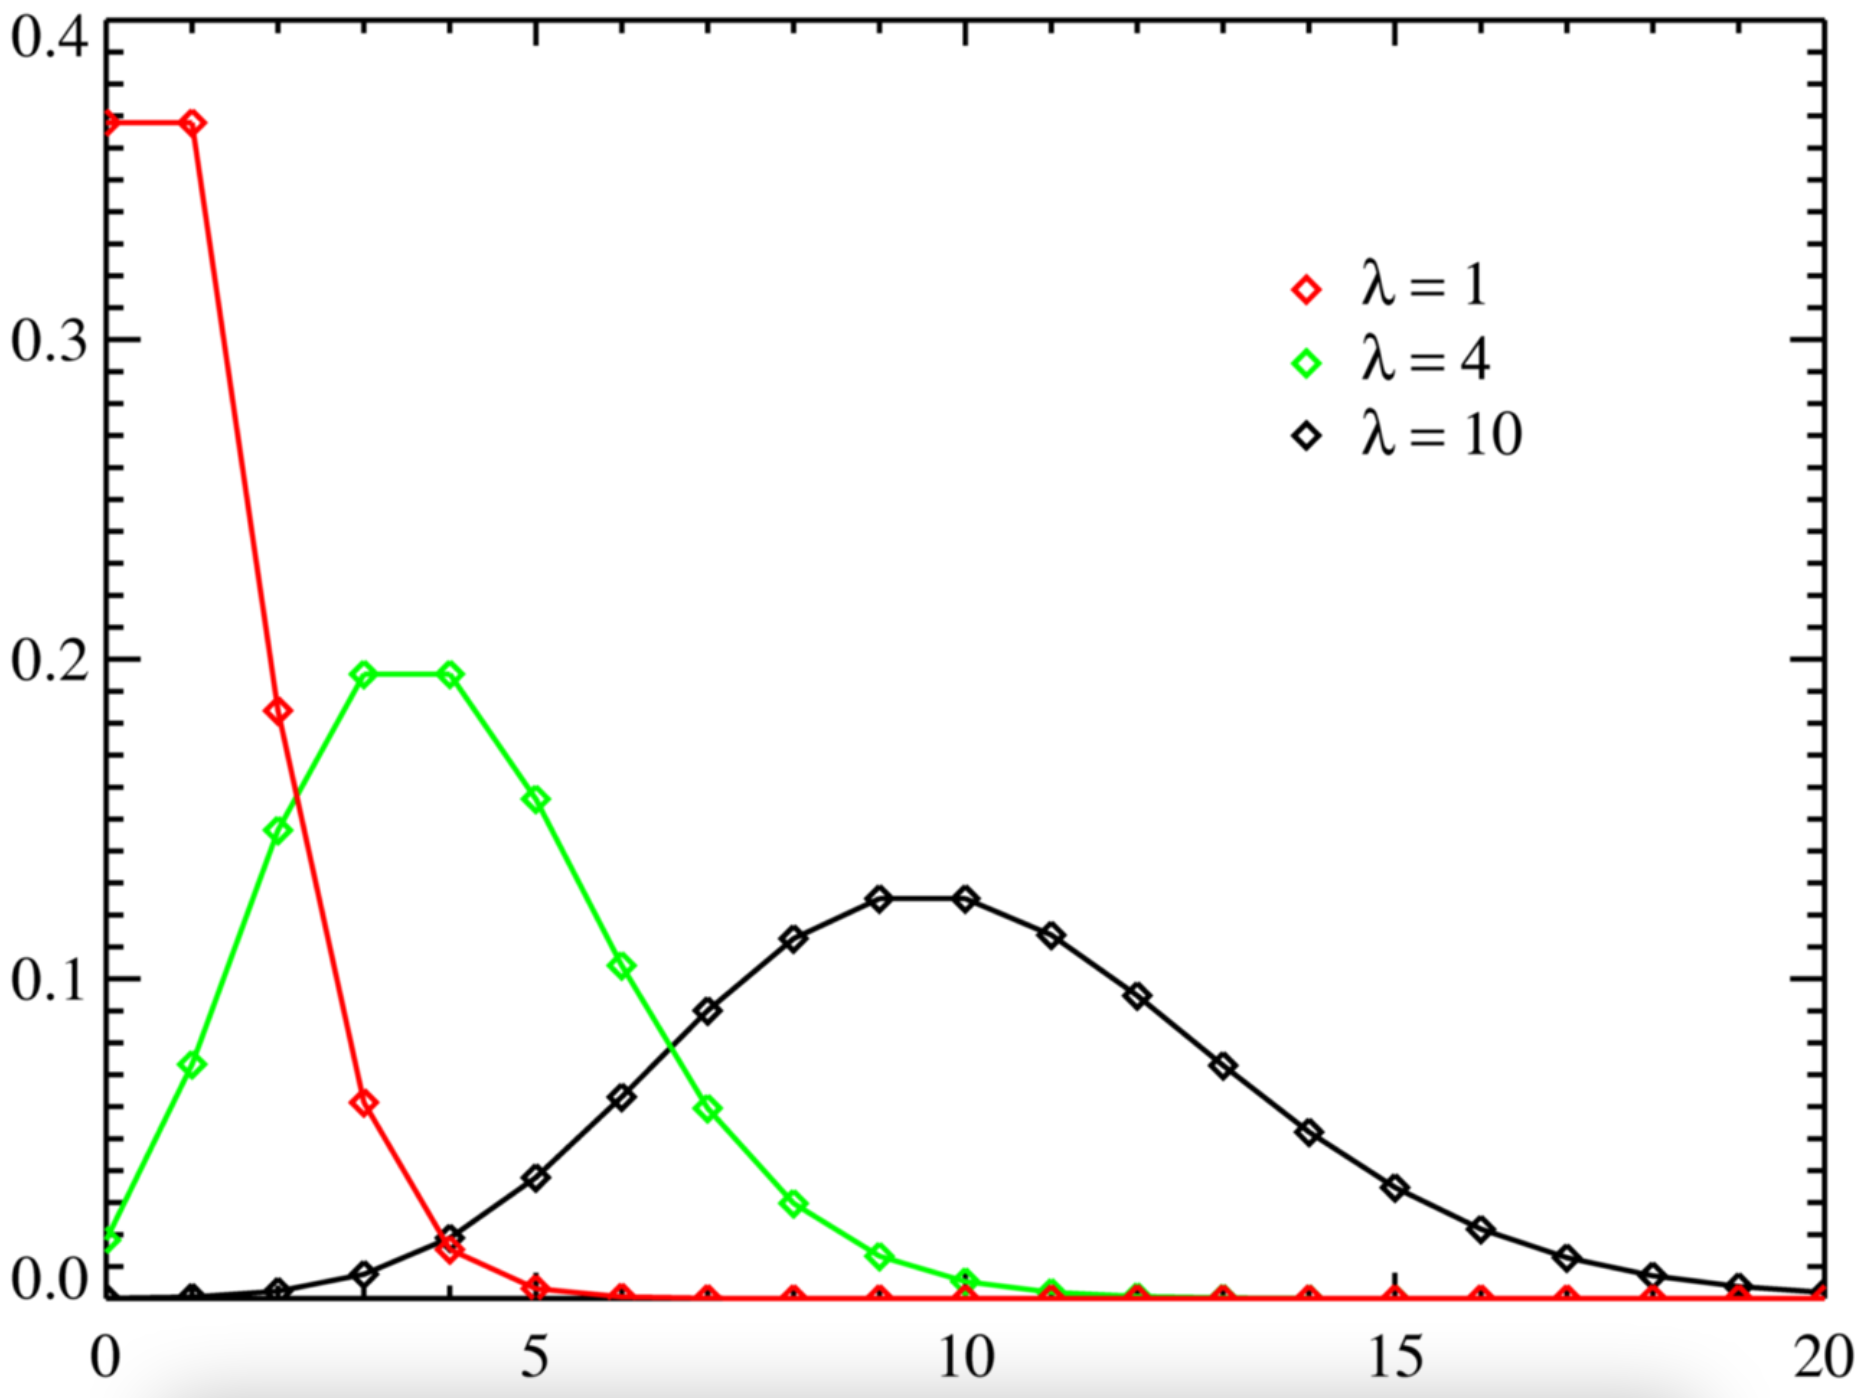
\includegraphics[scale=0.23]{pois}
	\end{center}
	
\end{frame}	

	\section{Negative Binomial}
\begin{frame} 
	\frametitle{\insertsection} 
	Negative binomial is a mix of poisson and Gamma distribution. 
	
	\begin{center}
		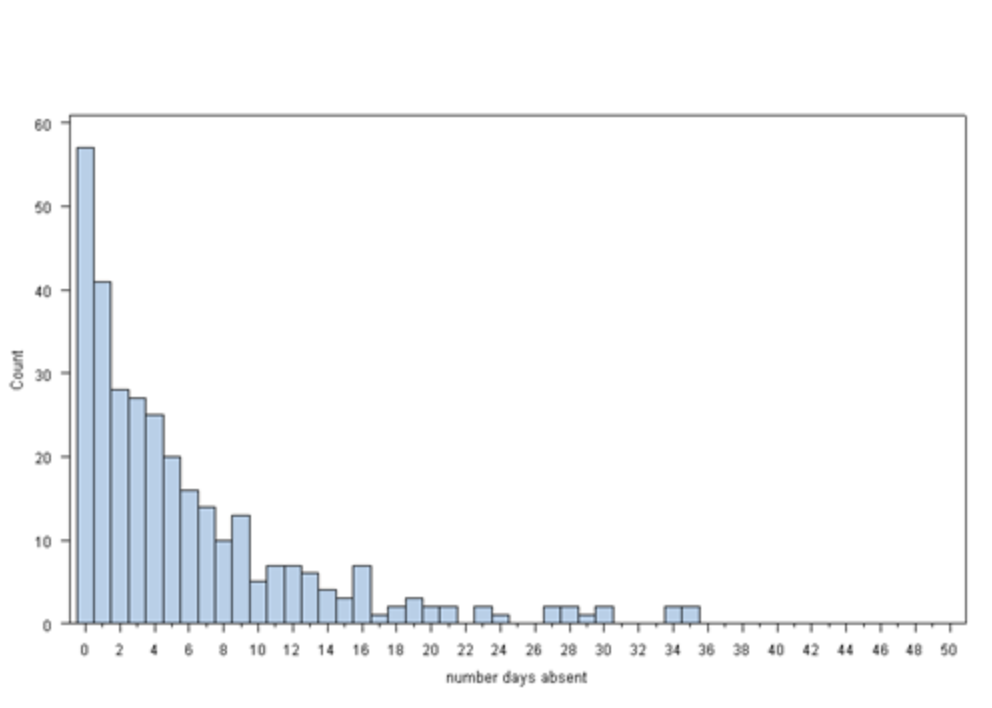
\includegraphics[scale=0.5]{neg_bin}
	\end{center}
	
\end{frame}	

\section{Output}
\begin{frame} 
	\frametitle{\insertsection} 
	
	\begin{center}
		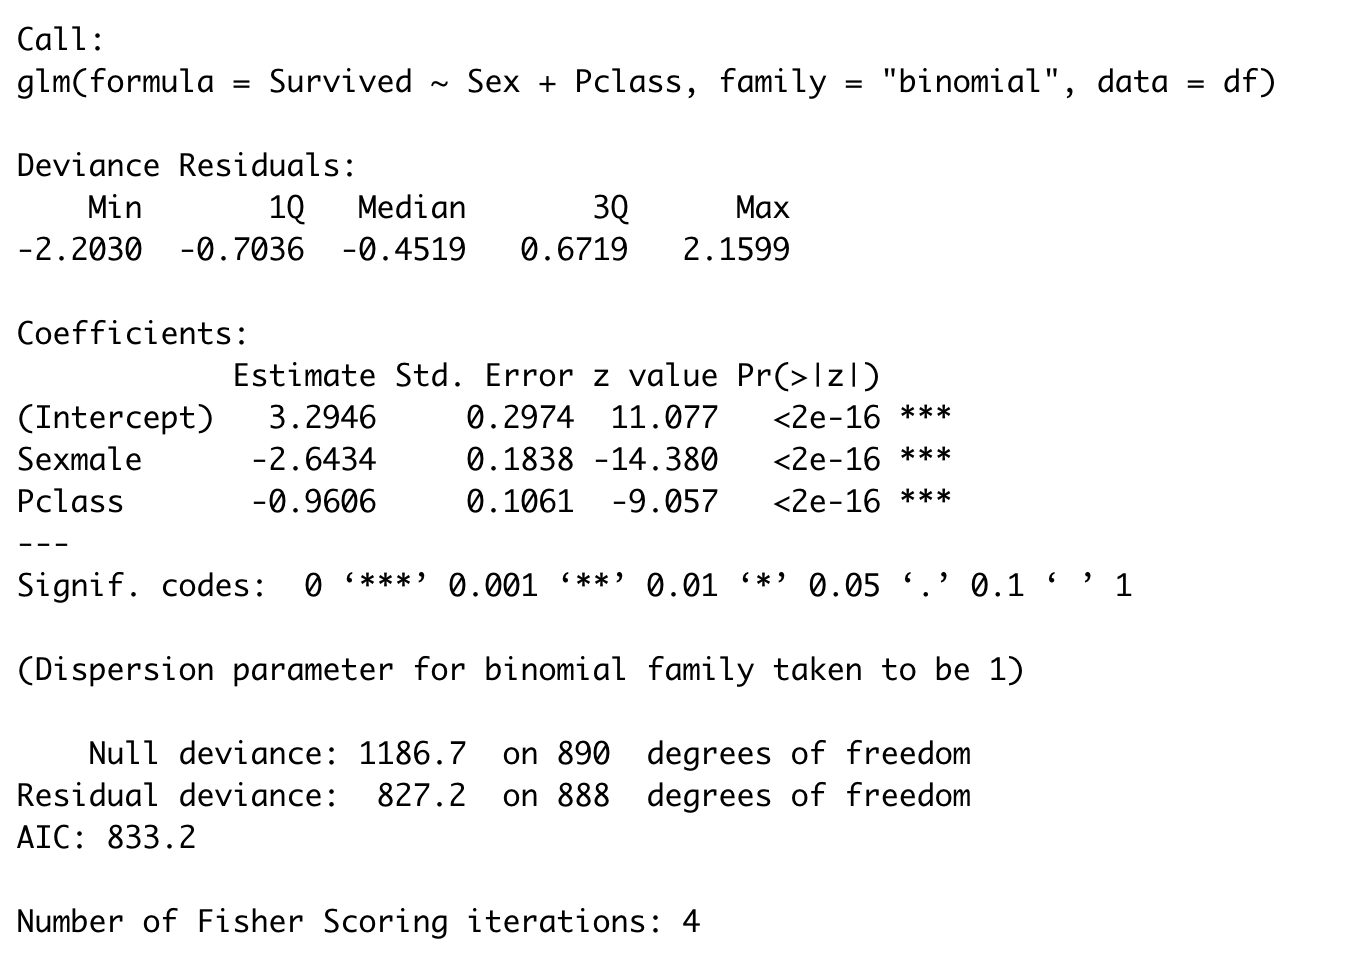
\includegraphics[scale=0.4]{logit1}
	\end{center}
	
\end{frame}	

\begin{frame} 
	\frametitle{\insertsection} 
	
	\begin{center}
		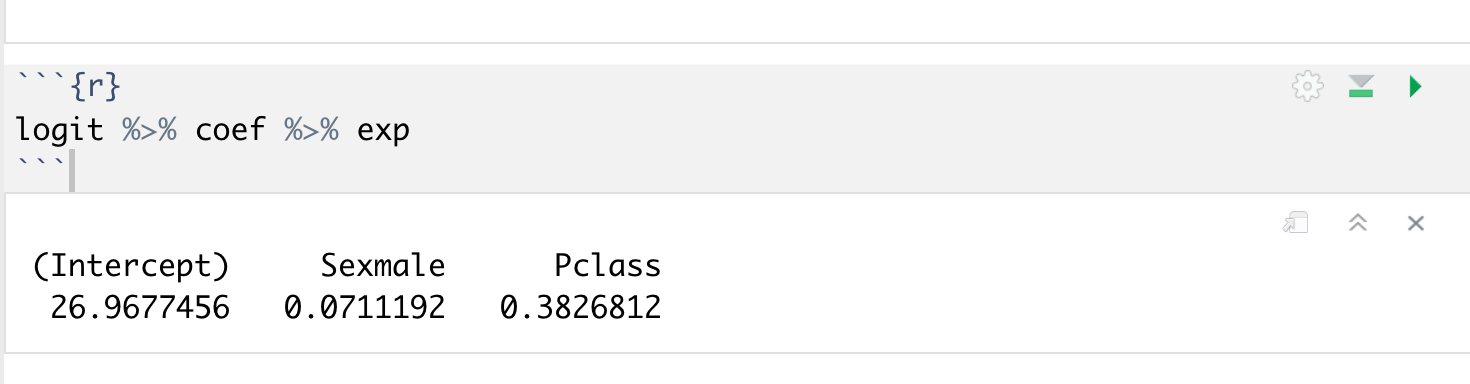
\includegraphics[scale=0.4]{logit2}
	\end{center}
	
\end{frame}	


\end{document}